% ================================================================================================================
%   ____ _____    _    _   _ _____  ______   ___   ___ _____                                     _              
%  / ___| ____|  / \  | \ | |_   _|/ /  _ \ / _ \ / _ \_   _|     __ _  ___  ___  _ __ ___   ___| |_ _ __ _   _ 
% | |  _|  _|   / _ \ |  \| | | | / /| |_) | | | | | | || |      / _` |/ _ \/ _ \| '_ ` _ \ / _ \ __| '__| | | |
% | |_| | |___ / ___ \| |\  | | |/ / |  _ <| |_| | |_| || |     | (_| |  __/ (_) | | | | | |  __/ |_| |  | |_| |
%  \____|_____/_/   \_\_| \_| |_/_/  |_| \_\\___/ \___/ |_|      \__, |\___|\___/|_| |_| |_|\___|\__|_|   \__, |
%                                                                |___/                                    |___/ 
% ================================================================================================================

\section{Представление геометрии в GEANT/ROOT}\label{sec:secGeoROOT}

Существует несколько способов задать геометрию для VMC-связки GEANT+ROOT --- с помощью текста (geo), с помощью XML в файле формата GDML, в виде макроса на языке ``C'', интерпретируемого системой ROOT и формирующего выходной файл (обычно --- .root, но возможно и .gdml). Также возможно использование какого-либо программного инструмента, некоторые из которых описаны в секции~\ref{sec:ExistSols}.

\subsection{Реализация CSG}\label{sec:secRootCsg}

% \todo переформулировать
Список реализованных в GEANT4 и ROOT примитивов совпадает практически полностью. В настоящее время в рамках проекта AIDA~\cite{AIDA} в ЦЕРН ведётся разработка пакета Unified Solids~\cite{USOLIDS}, ставящего своей задачей получить единое описание геометрии в пакетах GEANT4 и ROOT.

Для описания геометрических форм в пакетах GEANT/ROOT применяется CSG (см. секцию~\ref{sec:secGeoCSG}).
Алгоритмы проведения частиц, реализованные в GEANT/ROOT, оптимизированы для соответствующего описания геометрии, применяемого в этих пакетах.
Принимая во внимание тот факт, что геометрия в GEANT/ROOT нужна для выполнения моделирования взаимодействия частиц с материалом, можно сказать, что примитив --- это объект, имеющий геометрическое представление и для которого реализовано решение геометрических задач, возникающих при моделировании. Среди таких геометрических задач можно отметить задачу нахождения расстояния до ближайшей границы примитива от некоторой точки внутри объёма, в одном заданном направлении или в любом возможном направлении. Эту задачу необходимо решать многократно в процессе проведения частицы для того чтобы определить так называемый максимальный допустимый геометрический шаг. В результате моделирования физических процессов получается максимальный допустимый шаг из соображений физики. Для того чтобы собственно изменить координату частицы из этих двух шагов выбирается минимальный. Каждый примитив, как в GEANT4, так и в ROOT, реализован как отдельный C++ класс, имеющий свои геометрические параметры среди членов данных, и решение описанных выше геометрических задач среди методов. Следует, отметить, что есть только параметры примитива, но нет никакого описания типа BREP. Уравнения границ фигурируют лишь в неявном виде в коде методов для решения геометрических задач. Более подробно примитивы описаны в~\ref{sec:Primitives}.

% Перетащено из Boolean
При этом не требуется дополнительной реализации решения геометрических задач, т.к. удаётся комбинировать то, что реализовано в примитивах.
Особенности применения Булевых операций для задания формы объёма в ``CATIA-GDML geometry builder'' описано в~\ref{sec:Boolean}.

%Таким образом
Наблюдается некоторая аналогия между BREP и CSG, заключающаяся в том, что в любом случае сложное тело или базовый примитив имеет некоторые границы, заданные аналитическими выражениями. Корни этой аналогии лежат в фундаментальной математике. Однако решающая разница заключается в том, что для примитива эти границы чётко определены и имеется лишь ограниченное число параметров, позволяющих изменять форму примитива.

\subsection{Иерархия объёмов}\label{sec:secRootHierarchy}

% А первая --- это форма с помощью CSG, если чё.
Вторая составляющая геометрического представления в GEANT/ROOT это иерархия объёмов.
Введём понятия логического и физического объёмов, формы и материала. Логический объём (logical volume), или просто объём (volume) это базовый элемент для построения иерархии объёмов. Объём описывает непозиционированный объект и всё, что находится внутри него. Объём характеризуется формой (shape) и материалом (material). Форма --- это заданные с помощью CSG границы пространства, по методу, описанному выше. Материал включает в себя описание химического состава, плотности, и т.д. При помещении одного логического объёма в другой, например объёма $A$ в объём $B$, образуется так называемый физический объём (physical volume), или узел (node), $B_1$, который обозначает взаимоотношение $A$ и $B$ как материнский-дочерний и характеризуется некоторой матрицей $M_{B1A}$ позиционирования $B_1$ внутри $A$.

\begin{figure}[H]
\centering
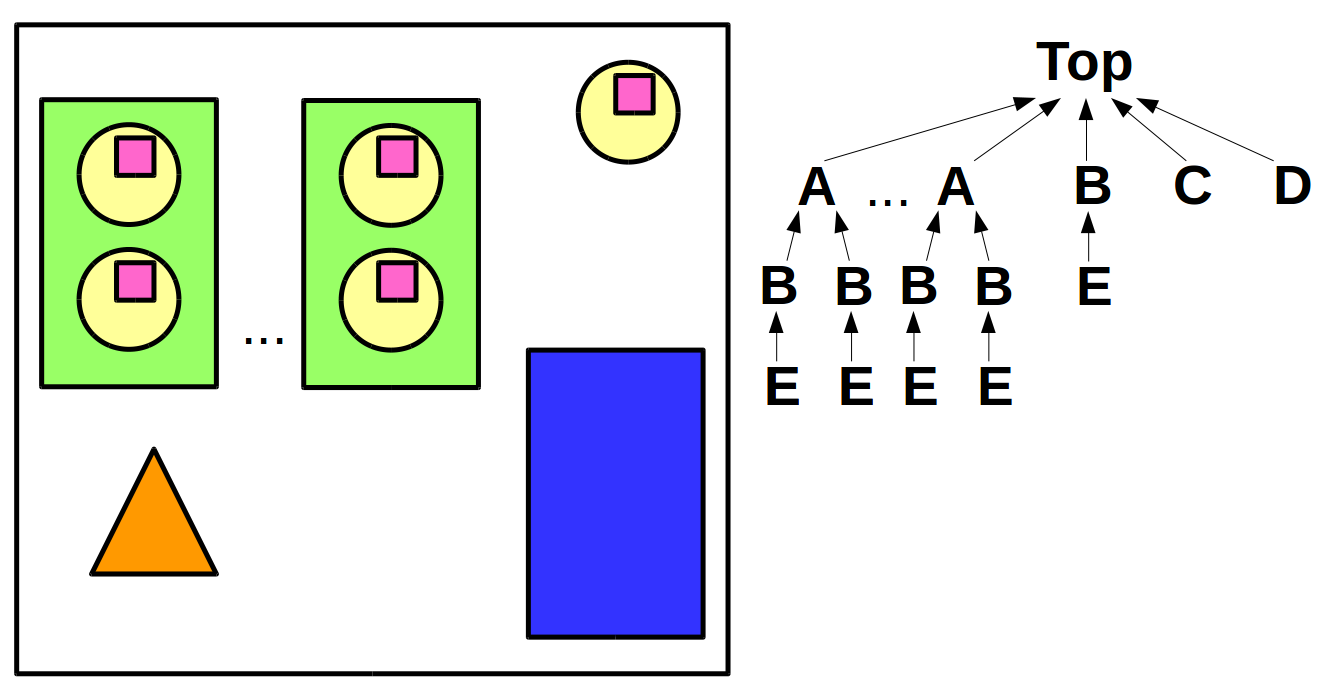
\includegraphics[width=0.7\textwidth]{pictures/ROOT_geo1.png}
\caption{Пример MC-геометрии, цвет означает материал. Полное дерево MC-модели (справа). Хранение такого полного описания геометрии невозможно из-за ограничения по памяти, однако часть дерева строится динамически по мере проведения частицы через геометрию.} % \todo
\label{fig:ROOTgeo1}
\end{figure}

\begin{figure}[H]
\centering
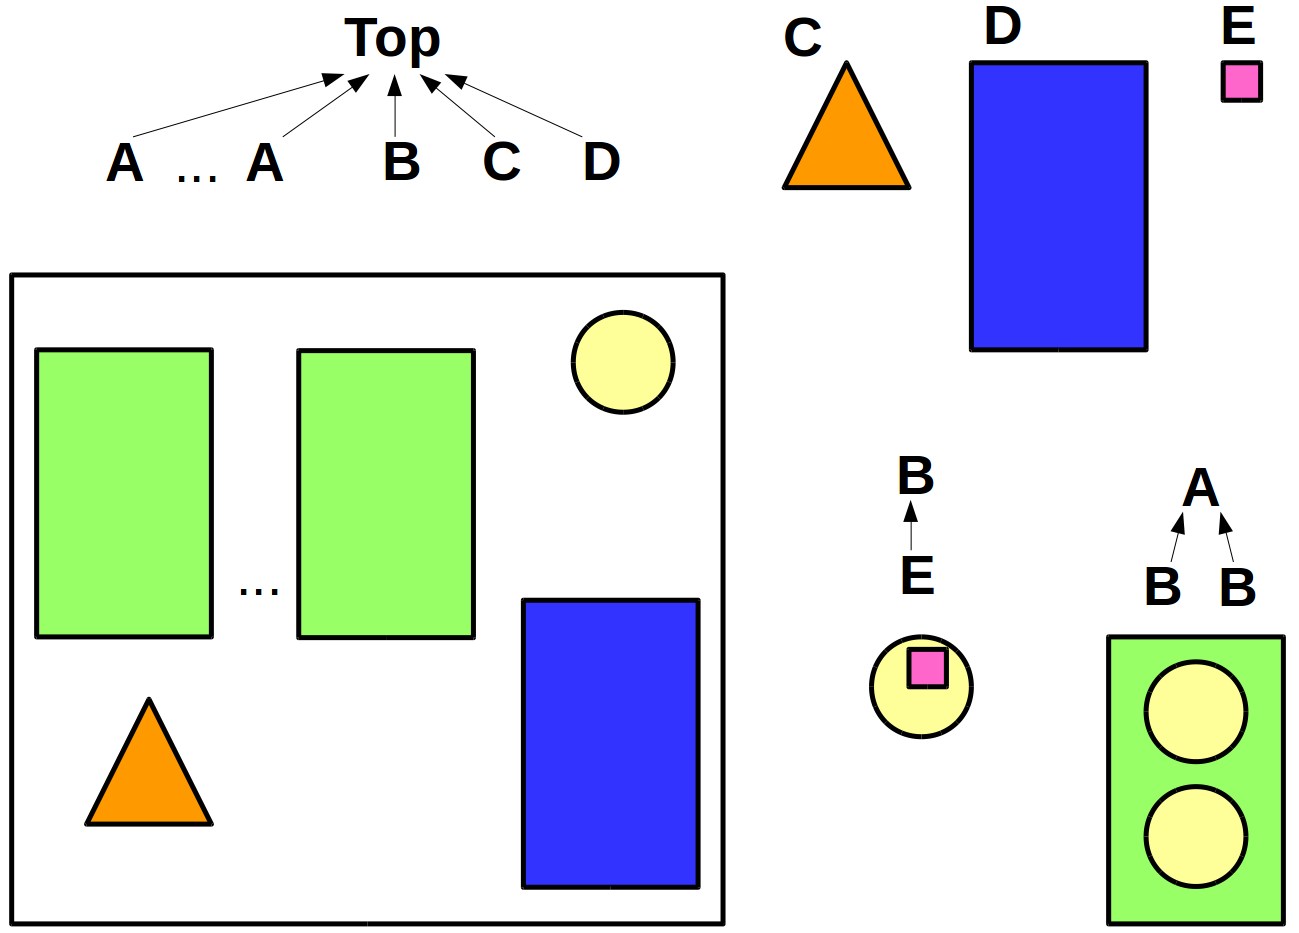
\includegraphics[width=0.7\textwidth]{pictures/ROOT_geo2.png}
\caption{Пример MC-геометрии, цвет означает материал. Более компактное эквивалентное описание той же геометрии, которое используется в системах проведения частиц ROOT и GEANT4. Сохраняются только локальные под-деревья --- взаимоотношения материнский-дочерний для одного уровня.} % \todo
\label{fig:ROOTgeo2}
\end{figure}

\begin{figure}[H]
\centering
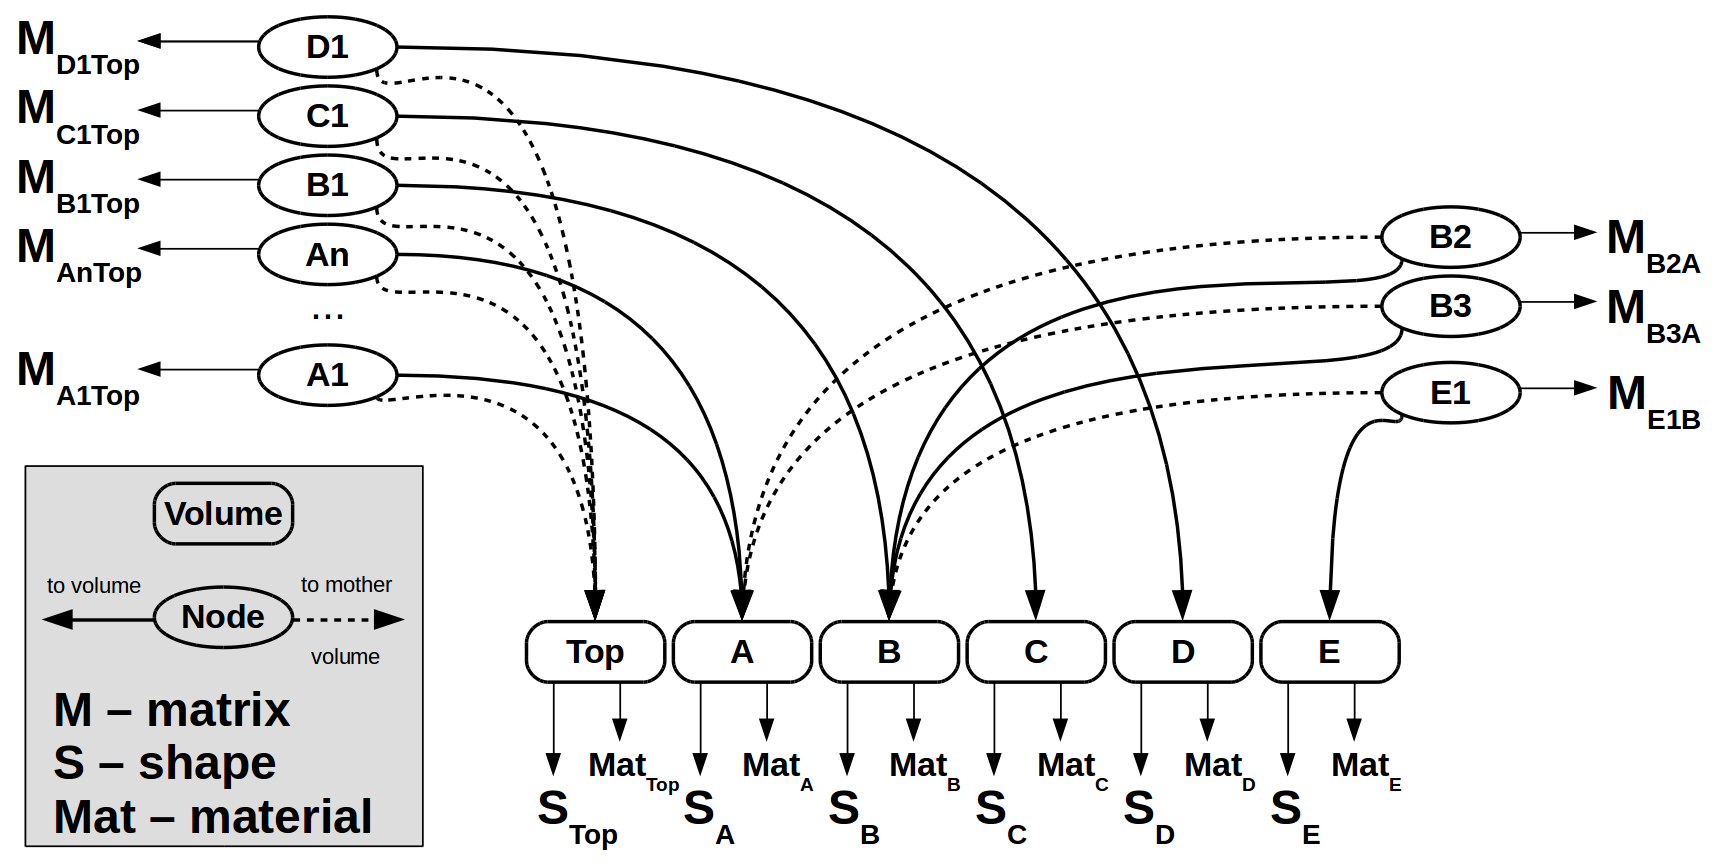
\includegraphics[width=0.7\textwidth]{pictures/ROOT_geo3.png}
\caption{ Эквивалентное представление данной геометрии с помощью объектов классов TGeo* в памяти ЭВМ. Стрелки обозначают указатели.} % \todo
\label{fig:ROOTgeo3}
\end{figure}

Принимая во внимание развитие вычислительной техники, в особенности резкое повышение производительности графических карт, их доступность широким массам, и вообще увеличение их значимости в вычислениях общего назначения, представляется возможным разработка новых алгоритмов проведения частиц через материал, учитывающих особенности геометрического представления в САПР.

Чем выше уровень подробностей в геометрической модели, применяемой для моделирования с помощью GEANT/ROOT, тем больше времени занимает это моделирование. Для оценочных расчётов удобно применять грубые модели, для точного определения каких-либо характеристик --- подробные модели. Поэтому принято иметь несколько MC-моделей одной и той же установки, имеющих разный уровень подробностей.
% упомянуть FastMC ?
В САПР подобная проблема решается другим образом. Так, например, в САПР CATIA~v5 присутствует возможность автоматического огрубления геометрической модели для снижения нагрузки на графический адаптер и повышения частоты кадров при динамической визуализации трёхмерных объектов. Это становится актуально, когда количество треугольников, которые необходимо визуализировать, составляет десятки миллионов.

% Asssembly-volume
\subsubsection{Assembly-volume}\label{sec:secAssemblyVolume}

В GEANT/ROOT существует тип объёмов, называемый Assembly, который характеризуется тем, что он не имеет формы и материала. Практически объём типа Assembly является контейнером без границ, который объединяет свои дочерние объёмы, что особенно удобно как минимум в двух случаях. Во-первых, если необходимо многократно позиционировать группу объёмов, которую невозможно охватить простой формой. Во-вторых, если преобразование координат при позиционировании одного или группы объёмов имеет сложную структуру и удобно представить его как суперпозицию двух преобразований.
%Как частный случай можно упомянуть ситуацию, когда какой-либо параметр преобразования является параметром модели (см. секцию~\ref{sec:Parameterization}).
% Написать про то, как позиционируется камера в газе рича. Есть один параметр - поворот - и чтобы его не использовать много раз при позиционировании всех кусочков, можно охватить кусочки асс-волюмом и крутить его.

% Replica
\subsubsection{Division/Replica}\label{sec:secDivisionReplica}

Одна из продвинутых возможностей геометрической подсистемы GEANT/ROOT --- это деление объёмов. В GEANT4 эта возможность называется replica, а в ROOT --- division. Суть заключается в том, что допускается деление некоторого объёма путём разрезания через равные промежутки вдоль одной из четырёх осей --- X, Y, Z и $\phi$, где $\phi$ --- круговое направление. В результате деления получается набор одинаковых под-объёмов --- долек, которые можно рассматривать как независимые вхождения одного объёма и позиционировать внутри другие объёмы. Отличие дольки от обычного объёма заключается в том, что для долек оптимизирована реализация проведения частиц. (\todo сформулировать лучше) Деление возможно только для ограниченного числа форм, таких, что все доли имеют одинаковую форму. Box --- в любом из трёх линейных направлений X, Y или Z. Tubs --- вдоль оси цилиндра, то есть вдоль линейной оси Z, или вдоль круговой оси $\phi$.

% ================================================================================================================
%   ____ ____  __  __ _     
%  / ___|  _ \|  \/  | |    
% | |  _| | | | |\/| | |    
% | |_| | |_| | |  | | |___ 
%  \____|____/|_|  |_|_____|
%                           
% ================================================================================================================

\subsection{Geometry Description Markup Language (GDML)}\label{sec:secGDML}

% \todo
В дополнение к форматам, перечисленным в секции~\ref{sec:secGeoFormats}, рассмотрим более подробно формат GDML~\cite{GDML}, применяемый для обмена GEANT/ROOT-геометрии в ``CATIA-GDML geometry builder''.

% \todo Ссылка на сайт
Язык разметки GDML разработан специально для обмена моделями представленными с помощью CSG с иерархией объёмов. GDML --- это XML-подобный язык. Файл на GDML имеет следующую структуру. Тэг верхнего уровня <gdml>, в нём 5 разделов:
<define>,
<materials>,
<solids>,
<structure>,
<setup>.

В секции <define> объявлены объекты, которые могут многократно использоваться в других секциях:
constant,
quantity,
variable,
position,
rotation,
scale,
matrix.
Все объекты должны иметь уникальные имена, определённые в значении аттрибута name. При работе с ``Builder'' используются лишь некоторые из перечисленных типов: variable, position, rotation. В ``Builder'' введено три объекта, которые всегда создаются в <define> секции: нулевой поворот ``identity'', нулевой сдвиг ``central'' и константа DEGtoRAD для перевода из градусов в радианы.

Секция <materials> предназначена для определения материалов, которые будут использоваться в модели. При описании логического объёма в секции <structure> должна быть ссылка на соответствующий тег <material> в секции <materials>.
% Кусок уехал в реализацию в билдере

В секции <solids> приведено описание форм логических объёмов. Как и в случае с материалами, в секции <structure>, при описании логического объёма должна быть приведена сслыка на соответствующий тег в секции <solids>.

Секция <structure> --- обычно самая большая секция, в которой описываются логические объёмы и их иерархия. Тег <volume> имеет как минимум два дочерних тега --- ссылка на материал <materialref> с аттрибутом ref, имеющим в качестве значения имя материала, определённого в секции <materials>, и ссылка на форму объёма <solidref> с аттрибутом ref, имещим в качестве значения имя формы, определённой в секции <solids>. Помимо этих двух обязательных дочерних тегов могу присутствовать другие теги, описывающие внутренний состав логического объёма. Самый распространённый случай --- тег <physvol>, обозначающий дочерний объём и имеющий аттрибут ref, указывающий на определённое ранее описание другого объёма.

Последняя секция <setup> служит для объявления одного логического объёма в качестве объёма верхнего уровня. Также здесь задаётся название установки, которое в CbmRoot должно быть FairGeom.
